% How to use R
% Author: Sam Pollard (sam.d.pollard@gmail.com)
% Last Modified: April 12, 2015

\documentclass[12pt]{article}
\usepackage[margin=1in, headheight=15pt]{geometry}
\usepackage{amsmath, amssymb, amsthm}
\frenchspacing % Single spacing after all periods.

% Remove the headrule and make enough space for the header
\usepackage{fancyhdr}
\renewcommand{\headrulewidth}{0pt}
\setlength{\headheight}{15pt} % If two lines in the header, make 30pt

\usepackage{graphicx, hyperref, fancyvrb}

\pagestyle{fancy}
\lhead{Learn you some R}
% If something is more than 1 page, add the page number. May require two compilations.
\usepackage{totcount}
\regtotcounter{page}
\cfoot{\ifnum\totvalue{page} > 1 \thepage \else\fi}

\newtheorem{exercise}{Exercise}

\begin{document}
\title{Learn you some R}
\author{Sam Pollard}
\date{\today}
\maketitle

\section{Introduction}

This guide is meant for people with little or no programming experience. That being said, this guide moves quickly and is aimed towards people who have spent a lot of time learning. There are many guides for programming which are aimed at computer scientists and use lots of jargon computer scientists have heard for years. This can be difficult to understand. On the other hand, many guides use such simple examples that you can't really do anything interesting with what you learn. This guide attempts to provide meaningful examples and explain the concepts which cannot be easily Googled. This guide comes with a supplementary R file which contains all of the example code used in this guide. If you have any feedback please mail me at \url{sam.d.pollard@gmail.com}

A word on notation: things written in \verb|this font| represent things which are typed exactly into R or the output of running commands. Things in \emph{this font} are either meant to be emphasized, vocabulary used by R, mathematical notation, or emphasis added by me. It should be clear from the context.

R is what is called an \emph{open} project. That means that anyone can contribute to R. This results in a large number of what are called \emph{packages}, which consist of a bunch of R files which ``work together'' to provide a service. This also results in R being really really huge in terms of the number of features it provides.

To install R, you must download it. I found the easiest way to do this is to go to \url{http://cran.cs.wwu.edu/}, which is hosted by WWU. You then install it like any normal program.

There are two basic ways to interact with R. One is in \emph{interactive} mode, the other is by executing a source file (called \emph{batch processing}). The latter can be done in Windows by clicking \emph{File} then \emph{Source R Code\dots}. Alternatively, you can edit an R source file by clicking \emph{File} then \emph{Open Script}. Interactive mode is useful for temporary or scratch work, while saving the commands you want to run into a text file and running them is more useful for automation and running experiments more than once.

Here is a sample run using interactive mode. As this guide progresses I recommend you execute each of the commands from the attached file \verb|sample_code.R|. Don't worry if much of this doesn't make sense; each component will be explained.

\begin{Verbatim}[frame=single, fontsize=\small]
> data(trees) # Load a sample dataset
> nrow(trees) # Count the sample size
[1] 31
> trees # Take a look at our data (Will print every row!)
> trees
   Girth Height Volume
1    8.3     70   10.3
2    8.6     65   10.3
3    8.8     63   10.2
         .
         .
 (Skipped for brevity)
         .
         .
30  18.0     80   51.0
31  20.6     87   77.0
> colnames(trees)
[1] "Girth"  "Height" "Volume"
> max(trees["Volume"]) # Find the largest in the column
[1] 77
> max(trees[3]) # The same as above because we access the third column
[1] 77
> apply(trees, 2, mean)
   Girth   Height   Volume 
13.24839 76.00000 30.17097
\end{Verbatim}
The \verb|[1]| symbol is a way of saying ``here is the first element of the output which you're not storing anywhere.''\footnote{Technically, it refers to the first element of a one-element vector. These will be explained later.} As we will see, it is common to store the output (or \emph{return value}) of a function call in a variable. This is explained in the next section, but in this example the return value of the function calls are just printed for the user to view.

It is important to keep in mind while programming R that almost everything is a function call. A \emph{function} is simply an object which takes in arguments and returns a value. For example, in math we write $f(x, y) = x^2 + y^2$ to describe a function $f$ which takes in two numbers and returns a third number. In R, we have something like \verb|nrow(trees)| which takes as input the variable \verb|trees| and returns the number of rows that variable contains. This is a general from of function calling, which follows the notation from mathematics: the function name followed by the arguments in parentheses. Functions are so important in R that after reading this guide the word ``function'' might sound weird.

There are some functions which take no arguments. For example, a useful function is \verb|data()|. Calling this function in the interpreter will open up a window which lists dozens of sample data sets, \verb|trees| being the one I chose for this guide.

The symbol \verb|>| is called a \emph{prompt}, which is the interpreter's (we'll define what that is later) way of saying ``I'm ready to process another command.'' Anything following a \# is a comment. This is to make the commands more human-readable, but are ignored by R entirely.

The last command is a bit complicated but fits with intuition. The \verb|apply| function takes as an argument some \emph{data frame} (in this case \verb|trees|), a 1 or 2 (1 for rows, 2 for columns), and a function (\verb|mean| here), and applies that function to each row or column in the data set. It is generally considered good practice to use built-in functions or ``one-liners'' such as \verb|apply| because they make code easier to understand and maintain.

\section{Basic Syntax and Examples}

R is what is called an \emph{interpreted} language. This means that there is an aptly-named \emph{interpreter} which keeps track of all the variables you have and how to execute the commands you run. The benefit to being interpreted is you have the flexibility of running one line at a time.

One potential drawback of an interpreted language is it can be difficult to find the errors in your code, because they may not show up until the source code is run. This can be mitigated by testing small chunks of your code as you write it.

In the first example, the object \verb|trees| is what is called a \emph{data frame}. In R, this is denoted \verb|data.frame|. This can be thought of as your typical spreadsheet format: A bunch of columns together. The one restriction is that each column must have equal length. Here is a quick example:

\begin{Verbatim}[frame=single, fontsize=\small]
> name <- c("H","He","Li")       # c can be thought of as "combine"
> mass <- c(1.0079,4.0026,6.941) # i.e. make a vector from the arguments
> atomic_number <- seq(1,length(name))
> mydf <- data.frame(atomic_number, name, mass)
> mydf                           # Print out the data.frame
  atomic_number name   mass
1             1    H 1.0079
2             2   He 4.0026
3             3   Li 6.9410
\end{Verbatim}

A few remarks are in order. First, the \verb|<-| symbol is used. This performs an \emph{assignment} of the right-hand value to the left-hand value. The \verb|<-| symbol is read as ``gets.'' This is the official way to do things, but you will often see code such as \verb|name = c("H","He","Li")| instead, which is also assignment (this is common syntax in other programming languages). I recommend using \verb|<-| because \verb|=| is used in another context in R, and it makes the distinction clearer. The fourth line calls the \verb|data.frame| function which takes as input some number of vectors and returns a data frame. This return value is stored in the variable \verb|mydf|.  The name, mass, and atomic\_number form the \emph{header} of the data frame. Sometimes data sets have headers, sometimes they don't. When loading in a csv you may specify whether you want R to try to put the first row as the header.

Unlike most other programming languages, the period can be used in variable names. It is typically used to denote a more specific way to go about things. For example, the function \verb|read| is used in a lot of contexts: It can be used to ask the user for input, it can read files, and many other things. A very useful ``version'' of \verb|read| is \verb|read.csv|, which takes in a csv file and turns it into a data frame.

Consider the following example, which will allow us to read in a csv and allow us to use all of R's features to analyze the data:

\begin{verbatim}
> mydf <- read.csv("report.csv", header = TRUE, sep = ",")
\end{verbatim}

The last argument is the \emph{separator}. This may be whatever you want. Cryptically, a csv (comma separated value) file may not be separated by commas. Oftentimes, it is tab-separated. To accommodate this, one can say \verb|sep = "\t"|. The backslash here \emph{escapes} the succeeding character \verb|t| and instead interprets this as a tab.

\section{Some Subtleties}
\subsection{Vectors}
The previous example used the \verb|c| function. The reason this is used is to put data in the correct format. This is an important part of R and programming in general. The distinction here is between a \emph{vector} and a \emph{scalar}. This fits with mathematical intuition but not so much with the real world. Ask a mathematician what a vector is and she will respond, ``It is something that behaves like a vector.'' While this is sort of a joke, there really isn't any better definition. In R, vectors are all over the place. Here are some examples and a non-example (can you spot which?)
\begin{Verbatim}[frame=single, fontsize=\small, numbers=left]
n <- nrow(trees)           # The number of trees
tag <- seq(1,n)            # A sequence from 1 to n, inclusive
lifespan <- 70*runif(n)    # Random values between 0 and 70, inclusive
volume <- trees["Volume"]  # The Volume of each tree
\end{Verbatim}

The last example is \emph{not} a vector. It is a data frame. This means things that require vectors won't work on the data frame. For example,
\begin{Verbatim}[frame=single, fontsize=\small]
> mean(volume)
[1] NA
Warning message:
In mean.default(volume) : argument is not numeric or logical: returning NA
\end{Verbatim}
However, if we make a small modification:
\begin{verbatim}
> volumevec <- trees[["Volume"]]
\end{verbatim}
This \emph{is} a vector.

If you're stuck, the \verb|class| function may describe what sort of data you're dealing with. Another useful method is \verb|ls()| which lists all the variables in your current workspace.

But what about the first example? Is it a vector? In some sense, yes. A vector can have one element. It is easiest to think of a scalar as the special vector which has one element. In general, most things you can do with scalars you can do with vectors. For example,
\begin{verbatim}
> lifespan <- lifespan + 15
\end{verbatim}
would increase the \verb|lifespan| variable by 15 (add 15 to each element in lifespan). Notice that this statement contains lifespan on the right-hand side and the left-hand side. In English we would say, ``take each element in lifespan and add 15 to it, storing the result in the variable lifespan.''\

\subsection{Building Up}
A common task when working with spreadsheets is combining data from multiple sources into a single structure. Here, we will look at the \verb|cbind|, and \verb|paste| functions. We will keep using our previous examples and create a data frame which represents all of the vectors we have created. We begin this somewhat contrived example by creating ``names'' for each of the trees.

\begin{verbatim}
> treenames <- paste("T", tag, sep = "")
\end{verbatim}

This creates a sequence of strings. Notice that R is smart enough to determine that while you only specified a single string ``T'' (instead of a vector of strings of the same length as \verb|tag|), it concatenates ``T'' with each element of \verb|tag|. For example, tree 15 would be named \verb|T15|.

Now, to create a new data frame from the existing data we created, try
\begin{verbatim}
> mydf <- cbind(treenames, trees, lifespan)
\end{verbatim}
This is close to what we want. The function \verb|cbind| takes as input data frames or vectors, and combines them \emph{by column} into a new data frame. There is an analogous function called \verb|rbind| which combines the data by row. Here is what the first few entries look like:

\begin{Verbatim}[frame=single, fontsize=\small]
> head(mydf)
  treenames Girth Height Volume lifespan
1        T1   8.3     70   10.3 15.18891
2        T2   8.6     65   10.3 15.85794
3        T3   8.8     63   10.2 15.41223
4        T4  10.5     72   16.4 15.30183
5        T5  10.7     81   18.8 15.86208
6        T6  10.8     83   19.7 15.87640
\end{Verbatim}
By the way, \verb|head| is a nice way to just see the beginning of a data frame (it is common to deal with thousands of rows of data). But this doesn't look quite right: the row names are just 1, 2, 3, \dots when we want them to represent our cleverly-named tree names. R allows us to change row names and column names using the aptly-named functions \verb|rownames| and \verb|colnames|. So,
\begin{verbatim}
> rownames(mydf) <- treenames
\end{verbatim}
We can also retrieve the row or column names by putting this function call on the right-hand side of an assignment like so: \verb|names <- rownames(mydf)|. To anyone with programming experience, this is a bit strange. The function can be used both as an \emph{l}-value, a.k.a. the left-hand side of an assignment statement a.k.a. the location of the variable getting changed) and an \emph{r}-value, a.k.a. the right-hand side of an assignment statement a.k.a. the return value of a function call. This is where the \verb|<-| notation keeps us sane: it directs us where the data we computed is being stored.

However, this data frame looks a bit strange:
\begin{Verbatim}[frame=single, fontsize=\small]
> head(mydf)
   treenames Girth Height Volume lifespan
T1        T1   8.3     70   10.3 15.18891
T2        T2   8.6     65   10.3 15.85794
T3        T3   8.8     63   10.2 15.41223
T4        T4  10.5     72   16.4 15.30183
T5        T5  10.7     81   18.8 15.86208
T6        T6  10.8     83   19.7 15.87640
\end{Verbatim}
So let's delete that first row:
\begin{verbatim}
> mydf <- mydf[,-1]
\end{verbatim}

That is some cryptic R code. There are other ways to accomplish the same task, but this one easily generalizes. In general, we access things by \verb|[row, column]|. So by default, we are accessing \emph{every} row. That is, there is nothing preceding the comma. Now, we are accessing every column but the first one (think of \verb|-| as removing the first column). Alternatively, we could \emph{include} every other column. So
\begin{verbatim}
> mydf <- mydf[,c(2,3,4,5)]
\end{verbatim}
would accomplish the same task. If we only cared about a few rows of \verb|mydf| we could write
\begin{verbatim}
> sample <- mydf[seq(4,9),]
\end{verbatim}
This takes the 4th through 9th rows of \verb|mydf|.

% \begin{exercise}
% Write your own \verb|head| function using what you know.
% \end{exercise}


\subsection{Default Parameters}
Returning to the first example of creating the tree names, we had to specify that \verb|sep = ""|, or the \emph{empty string}. If this was left out, i.e. \verb|paste("T",tag)|, then by default the strings are concatenated using a space as separator. We would get \verb|T 15| instead of \verb|T15|. Why is this? The motivation behind this is that most of the time a user will want the values separated by spaces. Without anything, there is the \emph{default parameter} for \verb|sep|, which is a space. Parameter specification takes the general form \verb|tag = value|. This is common notation, and \verb|=| is the character to use when specifying these parameters.

\section{Regression and Plotting}

This section will first gather some data and curves to be plot using R's regression features. These will be plotted but the output will be the default, plain format. Next, more advanced plotting features will be exploited to improve the quality of the figures and allow saving of the figures in multiple file formats.

\subsection{Regression}
Below is an extended example which plots a bunch of (simulated) noisy data and fits a curve to it. Which realistically is the solution to about half of all scientific problems.

\begin{Verbatim}[frame=single, fontsize=\small, numbers=left]
lb <- 0     # The lower and upper bounds will be used repeatedly
ub <- 10
time <- seq(from = lb, to = ub, length.out = 100)
noisy_data <- rnorm(100, mean = 0, sd = 5) + 10 # Equivalently: rnorm(100,10,5)
noisy_data <- abs(noisy_data) + time^2
# Make a scatterplot of the data
plot(time, noisy_data)
\end{Verbatim}

The first two lines create some made up data. Specifically, the ``noise'' is simulated with a normal distribution with mean 0 and standard deviation 5. Taking the absolute value of the data (\verb|abs| on line 5) will be nice a bit later when we want to interpret and plot the data. Since the 10 is added in line 4, this puts the mean at 15. Line 5 adds this noisy data to the square of a sequence of 100 elements going from 0 to 10. For example, \verb|time[1]^2 = 0|, \verb|time[2]^2 = 0.0102|, \dots, \verb|time[99]^2 = 97.99|, and \verb|time[100]^2 = 100| . We have seen \verb|seq| before and this is a more general use of the function. Squaring the points created from \verb|seq| gives points from the quadratic $f(x) = x^2$. Putting this all together means the noisy data \emph{should} be best fit by the curve $x^2 + 10$. Hopefully, a least-squares approximation will yield a curve close to that.

However, since we know from what distribution the data is sampled, we are dealing in some sense with a ``solved'' problem. Suppose for a while that we don't know the underlying distribution of the data. A valid technique would be to guess the data fits some linear model.

\begin{Verbatim}[frame=single, fontsize=\small, numbers=left]
linearmodel <- lm(noisy_data ~ time)
# Get the coefficients to overlay the best-fit line over the scatterplot
intercept <- coef(linearmodel)[1]
slope <- coef(linearmodel)[2]
curve(slope * x + intercept, add = TRUE)
\end{Verbatim}

Line 1 attempts to fit a linear model to the data. The \verb|~| character (tilde) indicates a \emph{formula} is used. With a linear model, the parameters are implied. That is, \verb|lm| reads in the simple expression \verb|noisy_data ~ time| and from it knows the data on which a regression should be performed and (among other things) \verb|lm| is attempting to find the best $m$ and $b$ which satisfy the equation $f(x) = mx + b$. Here, $m$ and $b$ are the \emph{coefficients}. Let's see how a linear model fits:

\begin{Verbatim}[frame=single, fontsize=\small]
> summary(linearmodel)

Call:
lm(formula = noisy_data ~ time)

Residuals:
    Min      1Q  Median      3Q     Max 
-16.658  -6.204  -1.393   6.674  21.740 

Coefficients:
            Estimate Std. Error t value Pr(>|t|)    
(Intercept)  -6.3943     1.8774  -3.406 0.000957 ***
time         10.0070     0.3244  30.852  < 2e-16 ***
---
Signif. codes:  0 ‘***’ 0.001 ‘**’ 0.01 ‘*’ 0.05 ‘.’ 0.1 ‘ ’ 1

Residual standard error: 9.458 on 98 degrees of freedom
Multiple R-squared:  0.9067,	Adjusted R-squared:  0.9057 
F-statistic: 951.8 on 1 and 98 DF,  p-value: < 2.2e-16
\end{Verbatim}
This summary is a Type I analysis of variance table. From this, we get a statistically significant result. To see this in more depth, we may call \verb|plot(linearmodel)| which produces several plots of the data. This further indicates the model is biased at the endpoints, suggesting a linear model isn't ideal.

To fit a nonlinear curve to the data we must use a different function, \verb|nls| (nonlinear least squares). Here is how that would be performed:
\begin{Verbatim}[frame=single, fontsize=\small]
quadratic <- noisy_data ~ p1*time^2 + p2
model <- nls(quadratic, start = list(p1=0, p2=0))
# Plot the new, least-squares quadratic
p1 <- coef(model)[1]
p2 <- coef(model)[2]
curve(p1*x^2 + p2, from = lb, to = ub, add = TRUE)
\end{Verbatim}
% To add:

% Plot & save plot output as NOT A PDF!
% Save output to a file
% The Resources section contains a link to a web page describing the \verb|par| function, which can be thought of as \emph{parameters} for plotting. Because of R's default function arguments, you will almost never have to worry about all of the dozens of parameters.

Now, analysis of variance is an incredibly sophisticated technique which I don't understand well. You'll notice that the nonlinear model does not provide the same depth of analysis with the call to \verb|summary| as the linear model. This is for good reason (see \cite{nlsanova}). However, in this case we can look at the plots and see that a quadratic model fits better.

\subsection{Plotting}
R has very powerful plotting features. They are described as ``beautiful'' by data visualization geeks. One reason for this is that R can output in vector formats, which is to say they scale to any size. There may be many more supported filetypes, but arguably the most important are png and pdf which this guide will explain.

This section will explain the various uses of the \verb|plot| and \verb|curve| functions used in the previous subsection and expand upon them to produce more sophisticated graphs.

Now, suppose we have already created all the required data and gone to assemble a plot like so: (this is simply a compilation of previously shown commands)
\begin{Verbatim}[frame=single, fontsize=\small]
plot(time, noisy_data)
curve(slope * x + intercept, add = TRUE)
curve(p1*x^2 + p2, add = TRUE)
\end{Verbatim}

The optional parameter \verb|add = TRUE| states that the curve should be added to an existing plot. The default is false, which is to say each call to \verb|curve| creates a new plot. Now, let's make these plots a bit nicer.

\begin{Verbatim}[frame=single, fontsize=\small, numbers=left]
pdf("sample_plot.pdf") 

# Make the scatterplot and label the axes
plot(time, noisy_data, xlab = "Time (months)",
     ylab = "Number of Cats (millions)")
# Change the title and marginal text
title("Number of Cats Over Time", line = 2, cex.main = 1.6)
mtext("What do we do with all these cats?\nBy Sam Pollard", font = 3,
      cex = 0.8)
# Overlay the linear and quadratic best fit curves
curve(slope * x + intercept, add = TRUE, lwd = 2, col = "red")
curve(p1*x^2 + p2, add = TRUE, lwd = 2, col = "blue")
# Create the legend
quadtext <- paste0(format(round(p1, 2), nsmall = 2), " t^2 + ",
                   format(round(p2, 2), nsmall = 2))
linetext <- paste0(format(round(slope, 2), nsmall = 2), " t + ",
                   format(round(intercept, 2), nsmall = 2))
legendtext <- c(quadtext, linetext)
legend("topleft", legend = legendtext, col = c("blue","red"), lwd = c(2,2))
# Say that we're finished plotting so the pdf can be saved
dev.off()
\end{Verbatim}

All this combined makes the nice graphic shown in Fig. 1.

\begin{figure}[h]
\centering
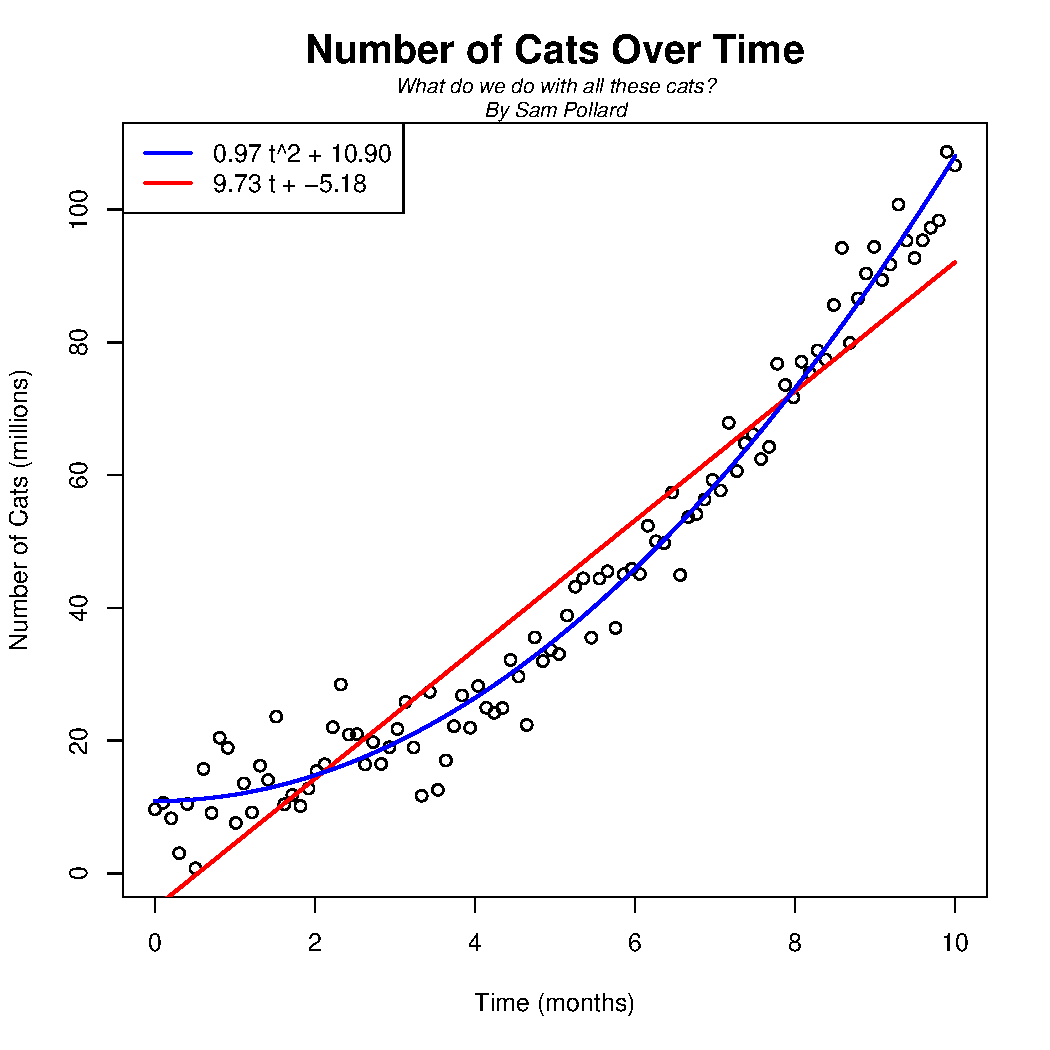
\includegraphics[scale=0.7]{sample_plot}
\end{figure}
% Other functions: axes
% TODO: Plot the R values, insert date in the corner, explain all the crazy code I just did.

\vfill
\section{Resources}
Arguably the most useful resource you can make use of in R is the \verb|help| function. You pass \verb|help| any function as an argument, which will direct you to an online help source. For example, \verb|help(rbind)|. This is the same as \verb|?rbind|.

Here are some other resources. I have not cited every one of the sources I used when creating this guide, but the ones omitted were generally answers from stack exchange or Wikipedia. Thus this can be also thought of as a partial bibliography.
\begingroup
\renewcommand{\section}[2]{}%
%\renewcommand{\chapter}[2]{}% for other classes
\begin{thebibliography}{}
	\bibitem{Learnxinyminutes}
		\url{http://learnxinyminutes.com/docs/r/}
		This is a pretty basic guide but is the easiest to follow.
		
	\bibitem{mycode}
		\url{https://github.com/sampollard/pcrystal}
		This is some of my own R source code.
		
	\bibitem{shortref}
		\url{http://cran.r-project.org/doc/contrib/Short-refcard.pdf}
		This is a useful cheat sheet. Much of it won't make sense right away, but will help you with commonly-used functions.
		
	\bibitem{rintro}
		\url{http://cran.r-project.org/doc/manuals/R-intro.pdf}
		This is a more in-depth guide to R. Notably, chapter 12 contains a lot of good information on graphics.
	
	\bibitem{nlsexample}
		\url{http://www.walkingrandomly.com/?p=5254}
		I used this reference in my nonlinear regression example.
		
	\bibitem{nlsanova}
		\url{https://stat.ethz.ch/pipermail/r-help/2000-August/007778.html}
		This contains a brief answer to why nonlinear models in R don't have the same analysis that linear models get.
	\bibitem{advgraph}
		\url{http://www.statmethods.net/advgraphs/} Provides explanation of many of the parameters of the \verb|par| and \verb|plot| functions.
\end{thebibliography}
\endgroup

\end{document}